% mycsrf 'for beeing included' snippet template
%
% (c) Karsten Reincke, Frankfurt a.M. 2012, ff.
%
% This text is licensed under the Creative Commons Attribution 3.0 Germany
% License (http://creativecommons.org/licenses/by/3.0/de/): Feel free to share
% (to copy, distribute and transmit) or to remix (to adapt) it, if you respect
% how you must attribute the work in the manner specified by the author(s):
% \newline
% In an internet based reuse please link the reused parts to mycsrf.fodina.de
% and mention the original author Karsten Reincke in a suitable manner. In a
% paper-like reuse please insert a short hint to mycsrf.fodina.de and to the
% original author, Karsten Reincke, into your preface. For normal quotations
% please use the scientific standard to cite
%


%% use all entries of the bibliography

\subsection{Laborejo ($\bigstar$)}

\parpic(2cm,2cm)[r][t]{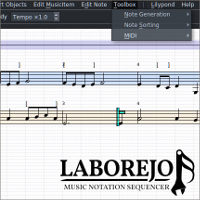
\includegraphics[width=1.8cm]{logos/laborejo-300dpi.png}}
\label{Laborejo}\acc{Laborejo} ist Teil einer Software Suite und sieht sich
selbst als \enquote{MIDI sequencer based on classical music notation}. Es ziele
hauptsächlich darauf, traditionelle Musik zu komponieren und zu produzieren.
Anders als andere Notationssysteme sei \acc{Laborejo} aber nicht dazu gedacht,
Notenblätter zu erzeugen, sondern auf und mit dem Rechner zu musizieren. Sein
Autor meint, dass man das Programm aus den Quellen oder als Paket seiner je
eigenen Distribution installieren könne.\footcite[vgl.][\nopage
wp.]{Hilbricht2019a} Ubuntu 18.04 offeriert tatsächlich ein Paket \acc{laborejo}
in der Version 0.8; die vom Autor angebene Downloadpage listet jedoch nur die
anderen Pakete der Software Suite, nicht \acc{laborejo}
selbst.\footcite[vgl.][\nopage wp.]{Hilbricht2019b}. Außerdem endet die
spezifizierte Handbuchseite in einer
'Hello-World'-Version.\footcite[vgl.][\nopage wp.]{Hilbricht2019c}

Neben diesen \acc{Laborejo}-Seiten gibt es noch ein
\acc{laborejo}-Github-Repository, das tatsächlich die Quellen der Software
anbietet. Die entsprechende Readme-Seite sagt ganz offen, dass es im Moment kein
Handbbuch und keine ordentliche Website gäbe, weil \acc{Laborejo} ein normales
Hobbyprojekt mit dem üblichen Problem sei, keine saubere Dokumentation erstellen
zu können.\footnote{\cite[vgl.][\nopage wp.]{Laborejo2018a}. Das Repository
enthält die GPL-3.0 unter dem Dateinamen \texttt{LICENSE}. \acc{Laborejo} ist
also freie Software.}

Mag all dies tatsächlich einer der speziellen Situation geschuldet sein, so
funktioniert doch auch die getestete Version nicht wirklich: Sie offeriert als
Import nur das Format \acc{Lisalo}, als Export u.a. die Formate \acc{PDF},
\acc{LilyPond} und \acc{MIDI}. Die eigentliche Noteneingabe erfolgt menue- und
tastaturbasiert, ist aber sehr unintuitiv arrangiert und ohne Handbuch nicht
nutzbar. Jedenfalls ist es uns nicht gelungen, unsere Referenzkadenz II
einzugeben -- und eben auch nicht zu importieren. Die neuere Version von Github
haben wir nicht einmal starten starten können.

Ohne dass das \acc{Laborjo} weiter ausreift, bietet es zu dem, was wir suchen,
keine Alternative, insbesondere für Musikwissenschaftler nicht: Zu flach ist die
Lernkurve, zuviele 'Try-and-Error'-Erkundungen sind nötig. Mag die Grundidee
auch jetzt schon anziehend sein, so muss die Umsetzung aber noch deutlich
reifen. Die bloße Möglichkeit soll uns ber noch einen Stern wert sein.
% this is only inserted to eject fault messages in texlipse
%\bibliography{../bib/literature}
